\documentclass[12pt]{article}
\usepackage{amsmath}
\usepackage{amssymb}
\usepackage{amsthm}

\usepackage{enumitem}
\usepackage{mathtools}
\usepackage{graphicx} % more modern
%\usepackage{epsfig} % less modern
\usepackage{subfigure} 
\usepackage{url}
\usepackage{amssymb, amsmath, amsthm}
\usepackage{float}

\newcommand{\leftcodemean}{{\langle\;\!\!\!\langle}}
\newcommand{\rightcodemean}{{\rangle\;\!\!\!\rangle}}
%\newcommand{\codemean}[1]{\leftcodemean #1 \rightcodemean}
%\newcommand{\expmean}[1]{\lvert #1 \rvert}
\newcommand{\commean}[1]{\lvert #1 \rvert}
\renewcommand{\emptyset}{\{\}}
\newcommand{\inl}[1]{{\bf inl}\;#1}
\newcommand{\inr}[1]{{\bf inr}\;#1}
\newcommand{\sumcase}[5]{{\bf sumcase}\ #1\ {\bf of}\ \inl{#2} \Rightarrow #3 \,{\bf |}\, \inr{#4} \Rightarrow #5}
\newcommand{\inj}{\iota}
\newcommand{\tymean}[1]{\llbracket #1\rrbracket}
\newcommand{\expmean}[1]{\llbracket #1\rrbracket}
\newcommand{\nsqsubseteq}{\not\sqsubseteq}
\newcommand{\listcase}[5]{{\bf listcase}\ #1\ {\bf of}\ {\bf nil} \Rightarrow #2 \,{\bf |}\, {\bf cons}(#3, #4) \Rightarrow #5}
\newcommand{\listcaseml}[5]{\begin{array}[t]{@{}l}%
                            {\bf listcase}\ #1\ {\bf of} \\%
                            \;\; {\bf nil} \Rightarrow #2 \\%
                            {\bf |}\, {\bf cons}(#3, #4) \Rightarrow #5%
                            \end{array}}
\newcommand{\envmean}[1]{\llbracket #1 \rrbracket}
\newcommand{\cross}{\times}


\title{ {\bf   Parallel Algorithm Benchmarking on BlackLight }\\
Early NUMA Benchmarks
} 
\author{Aapo Kyrola}

 
\begin{document} 
 \maketitle

\section{Introduction}

As part of Guy Blelloch's project "Problem Based Benchmark Suite (PBBS)", we are studying how a selection of  fundamental computer science algorithms (such as sorting, nearest-neighbor, graph algorithms) could be implemented efficiently on a supercomputer with Non-Uniform Memory Access (NUMA) shared address space.  Pittsburgh Supercomputer Center (PSC) kindly allocated us research time for their new Blacklight supercomputer (\url{http://www.psc.edu/machines/sgi/uv/blacklight.php}).

To begin our research, I wrote simple tests to measure the memory access latency on Blacklight. These results are inspired on Yucheng Low's similar results, but are based on my own code. I also implemented a simple extensible C++ ``framework" for implementing easily similar experiments. 

\section{Benchmark: NUMA {\it read} performance}

In the first round of experiments I tested read performance between threads. For threading, I used PThreads under C++. 
The basic anatomy of a test was as follows:  (1) each thread allocates 128 megabytes of memory and writes a sequence of integers to this data; (2) threads read data written by other threads. I did experiments with both sequential reading (i.e one thread reading a time) and parallel reading.  In each of the tests, I sum the integers read from the data. Although this is not necessary, this was done to prevent a smart compiler noticing that the code was not actually using the data it read.

\subsection{Experiment:  Sequential read}

This experiment used just one thread a time to read data. Therefore, there should be no congestion caused by our own software (it is unclear how {\emph software by other users} affects the memory system performance). 

\begin{figure}[H]
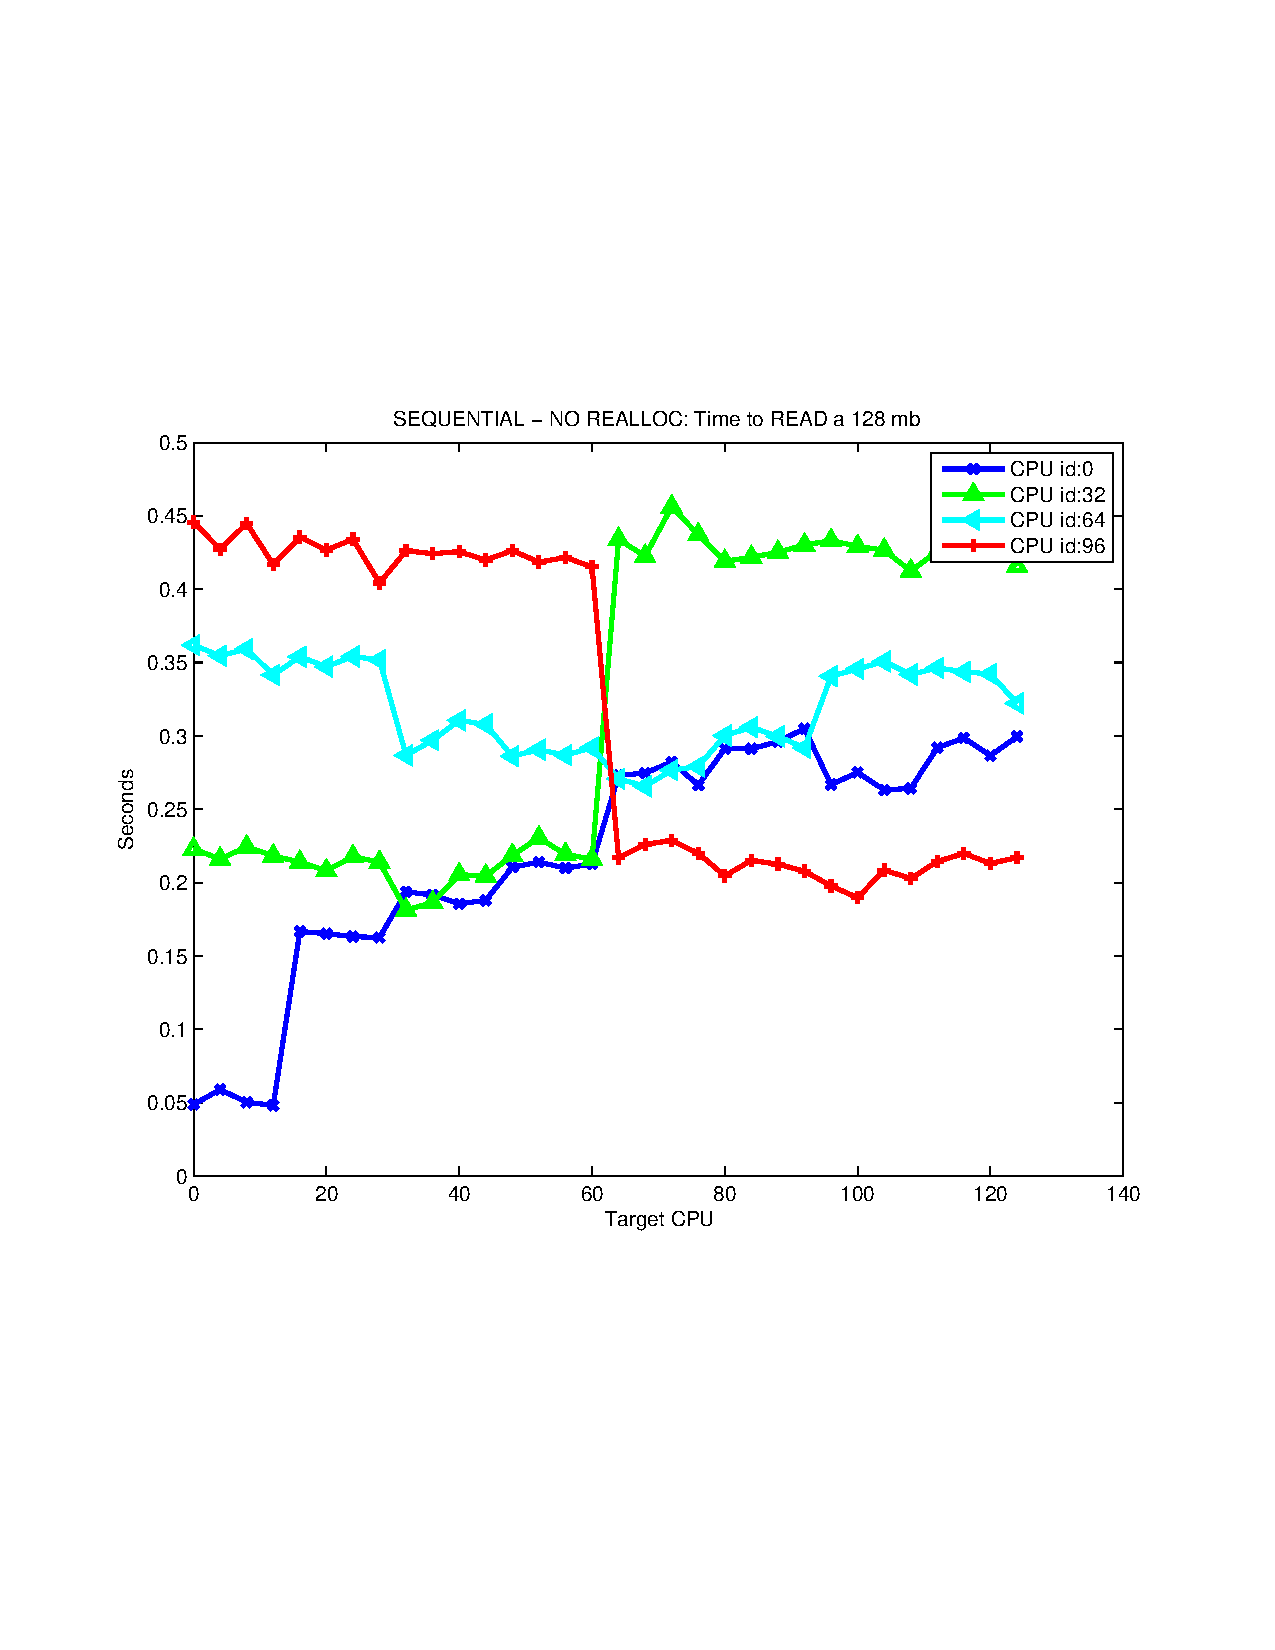
\includegraphics[width=0.95\textwidth]{blacklight_seq_access_norealloc.pdf}
\caption{Sequential read experiment with total number of 128 threads. Each curve shows the time used for reading a every 16th integer of a 128-megabyte array allocated by thread number corresponding to the x-axis. Curves for threads 0, 32, 64 and 96 shown. In this case, memory was not reallocated after each test. Curiously, the shape for thread 0 is very different. See the text for discussion.
}
\label{figseq1}
\end{figure}

Figure \ref{figseq1} shows the timings for the first experiment. Curiously, only thread 0 has sigfinicantly faster time to load its \emph{own} data!  This leads to following hypothesis: 


\smallskip
\framebox{
\parbox{0.9\textwidth}{\textbf{Hypothesis: } When cpu A allocates a chunk of memory, it is allocated to cpu A's memory. But when this chunk of memory is accessed by another cpu, B, Blacklight's memory system moves the data to this cpu's memory. }
} \\


That is, because thread (cpu) 0 is run first, all memory it accesses is actually moved to cpu 0's memory, or vicinity. When thread 32 is run for the same experiment, all its memory access is remote to cpu 0.

To test the hypothesis, I repeated the test but \emph{reallocated the data before each test}. That is, before running thread 32 after thread 0 had finished, I reallocated all integer arrays. See Figure \ref{figseq2}. Now each cpu has similarly shaped access pattern.

\begin{figure}[H]
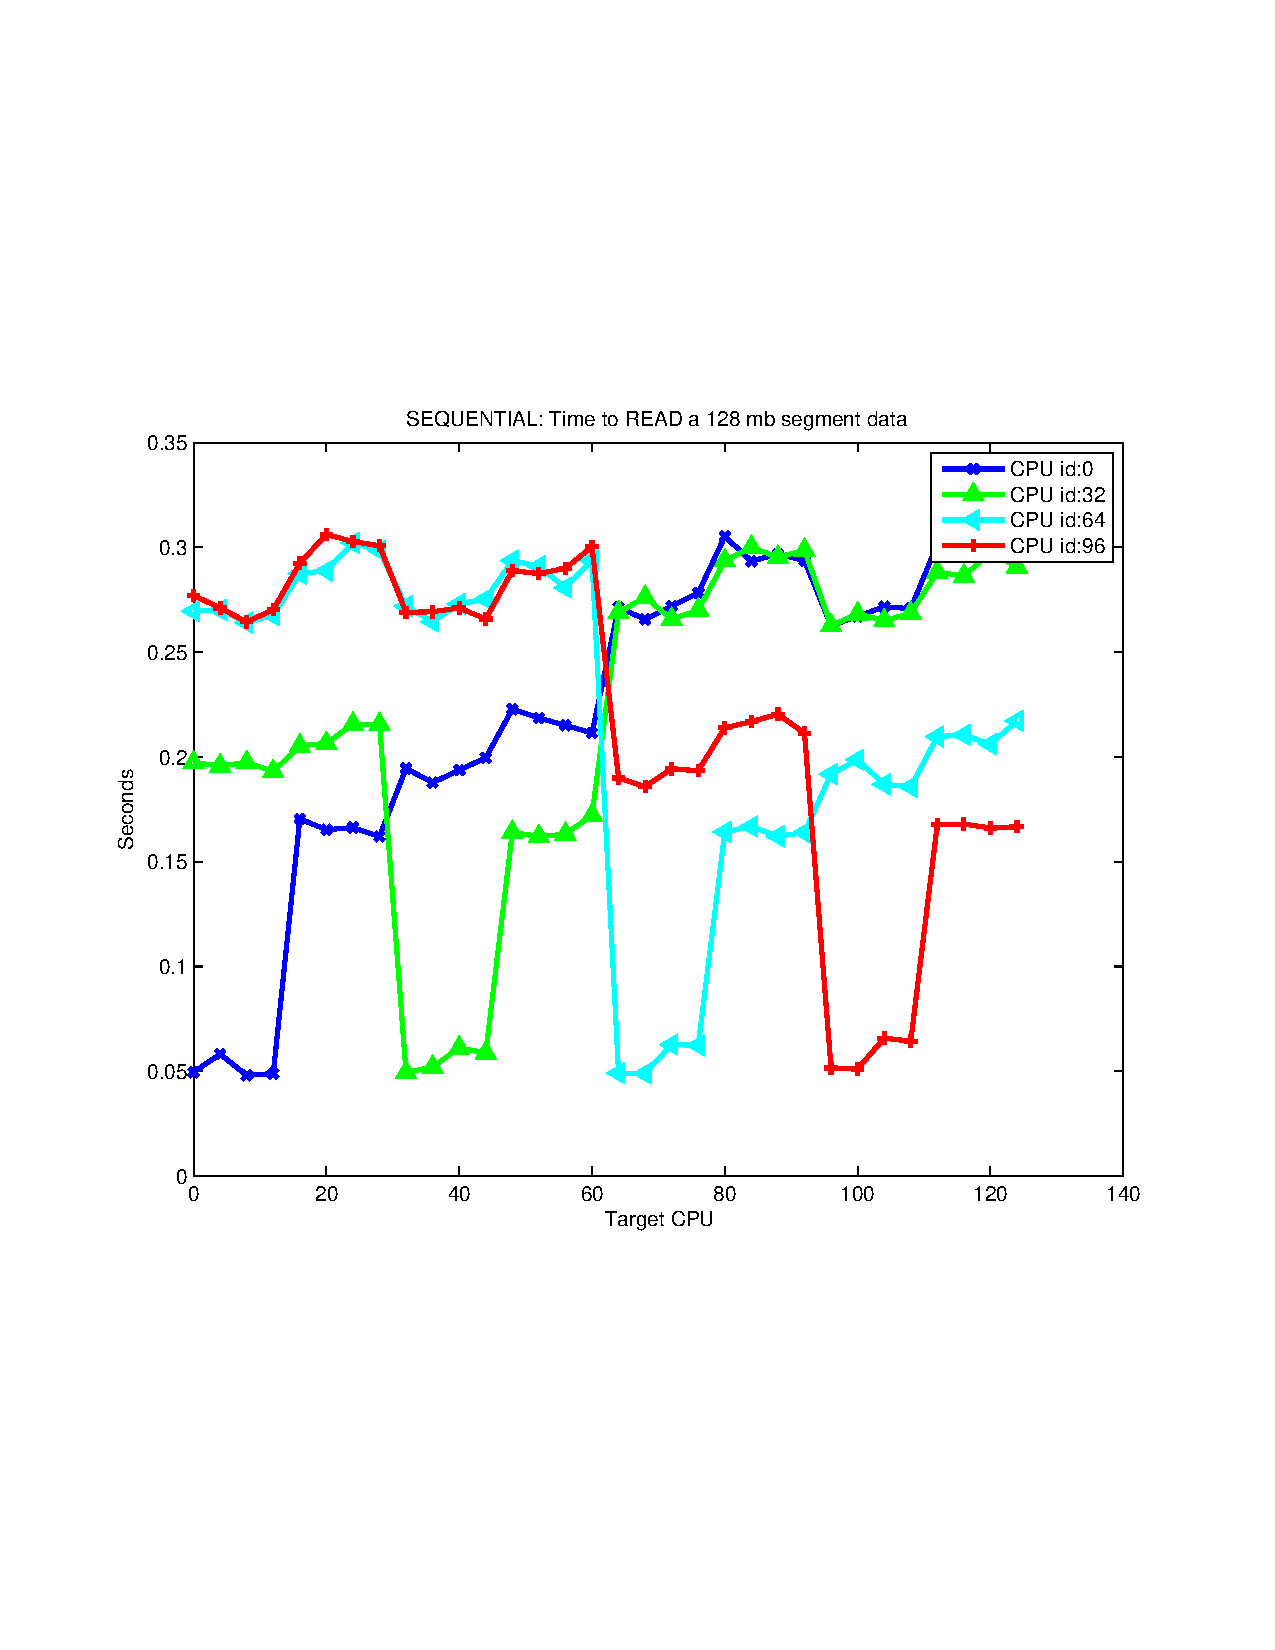
\includegraphics[width=0.85\textwidth]{blacklight_seq_access.pdf}
\caption{Sequential read experiment when data is reallocated before each round. Now each cpu can clearly access their data faster.
}
\label{figseq2}
\end{figure}


To further test the experiment, I made a very simple test:

Processor 54 allocated 1 gigabyte of memory, let's call it X. After that, following steps were taken (in sequence), 
with timings:

\begin{enumerate}
\item 54 read X:  0.384 secs

\item 4 read X: 2.366 secs

\item 4 read X again: 2.38 secs

\item 54 read X: 2.2 secs

\item 54 read X again: 0.39 secs
\end{enumerate}

This actually implies that the hypothesis must be \emph{rejected} because otherwise the second read by CPU 4 would had
been fast. Instead, it seems that the next time 54 needs to read the data, it must consult CPU 4 (or the memory system) on whether
CPU 4 had done something to the data. However, since the time is so long (2.2 secs), there probably has to be some data
transfer happening as well. And indeed, when test was executed with 128 megabyte chunk, the ratios of times were similar.

\subsection{Experiment: Parallel read}

Next test run 128 threads in parallel, each accessing a memory segment simultaneously. Experiment was run in lockstep: first each thread accessed its own array, on next step array of (cpu+1) mod 128, etc. Since each cpu first accesses its own array, it is faster than other remote accesses. 

\begin{figure}[H]
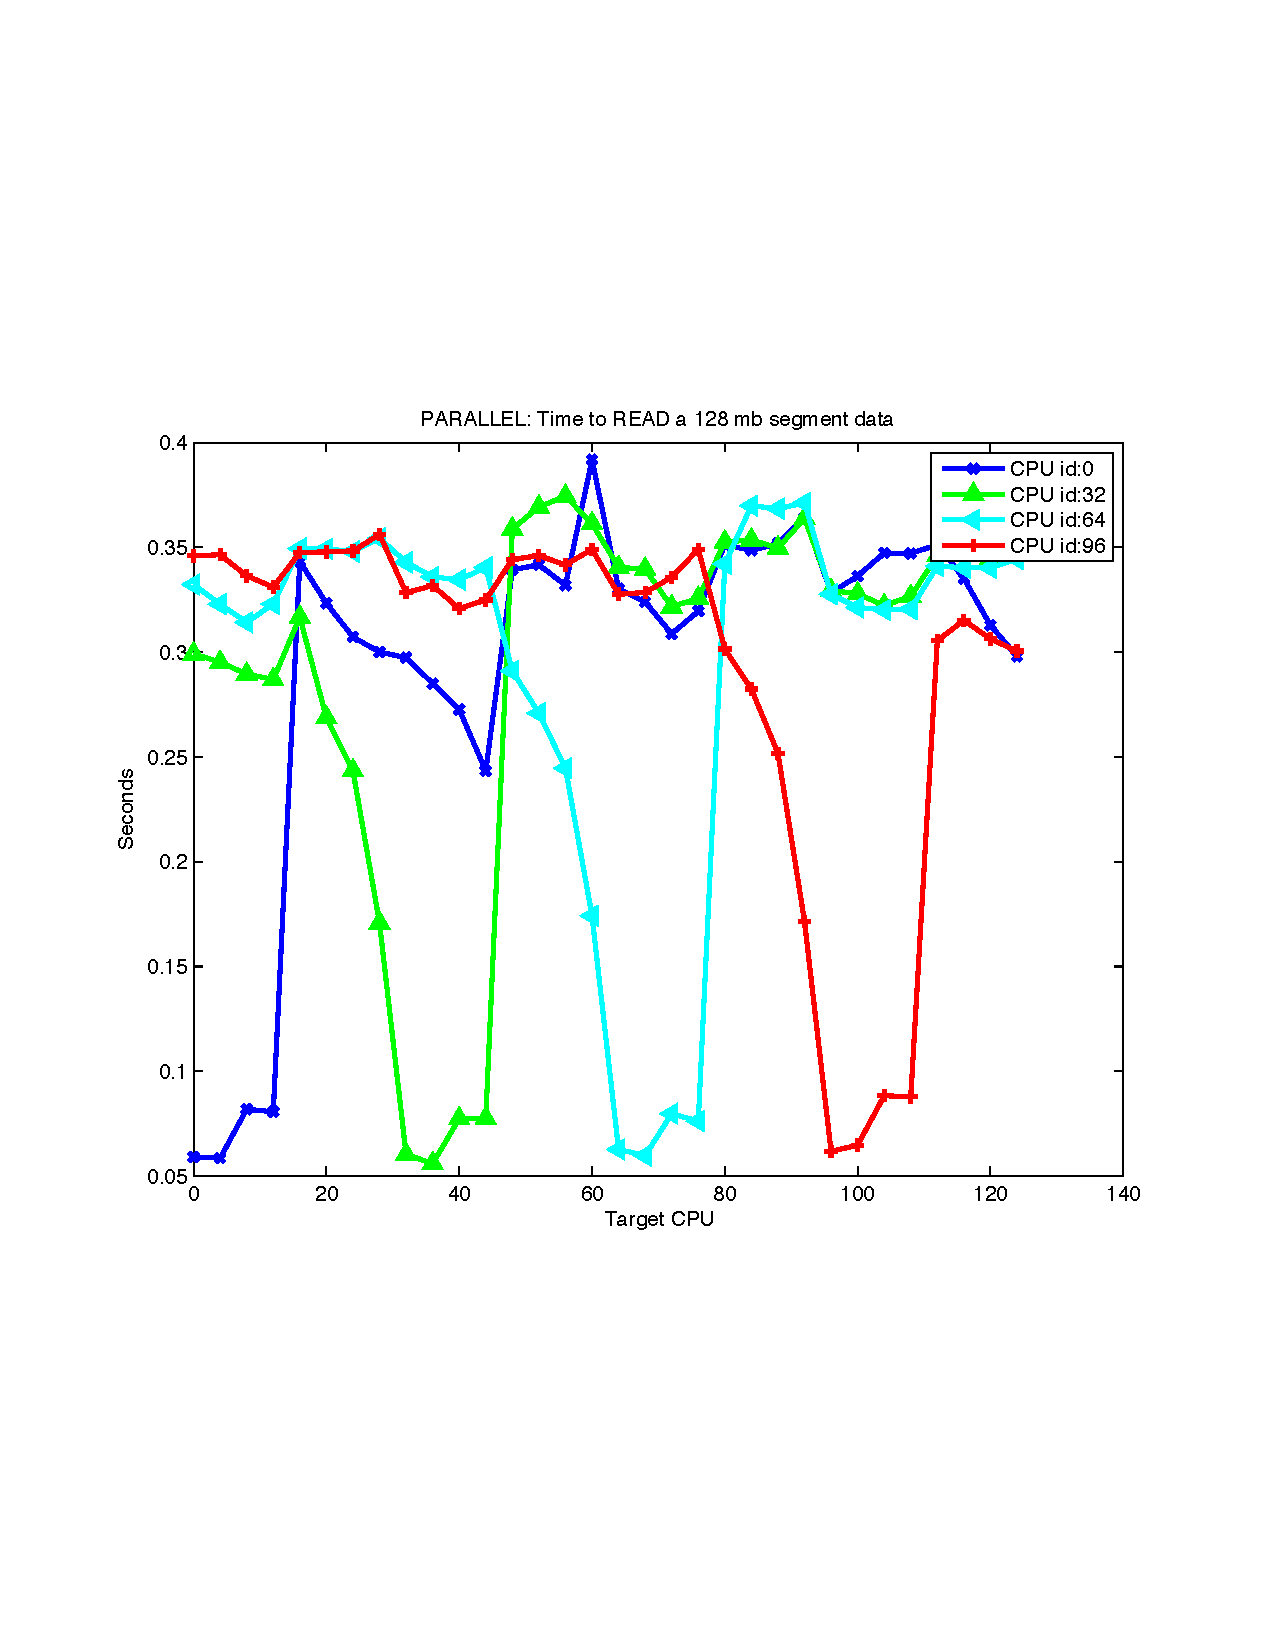
\includegraphics[width=0.95\textwidth]{blacklight_par_access.pdf}
\caption{Parallel read experiment with total number of 128 threads. Each curve shows the time used for reading a every 16th integer of a 128-megabyte array allocated by thread number corresponding to the x-axis. Curves for threads 0, 32, 64 and 96 shown. All 128 threads run in parallel, in steplock, accessing memory allocated by cpu, cpu+1, cpu+2, ... cpu+127. Before each step, data was NOT reallocated.
}
\label{figseqpar}
\end{figure}

\subsection{Experiment: Random access}

Next I run another sequential experiment, but instead of reading the integer array serially, it was accessed by jumping around
it. Figure \ref{figseqran} shows the results. Access times are about twice longer than with serial access for both local and remote acess.
This highlights the need for good  locality. 

\begin{figure}[H]
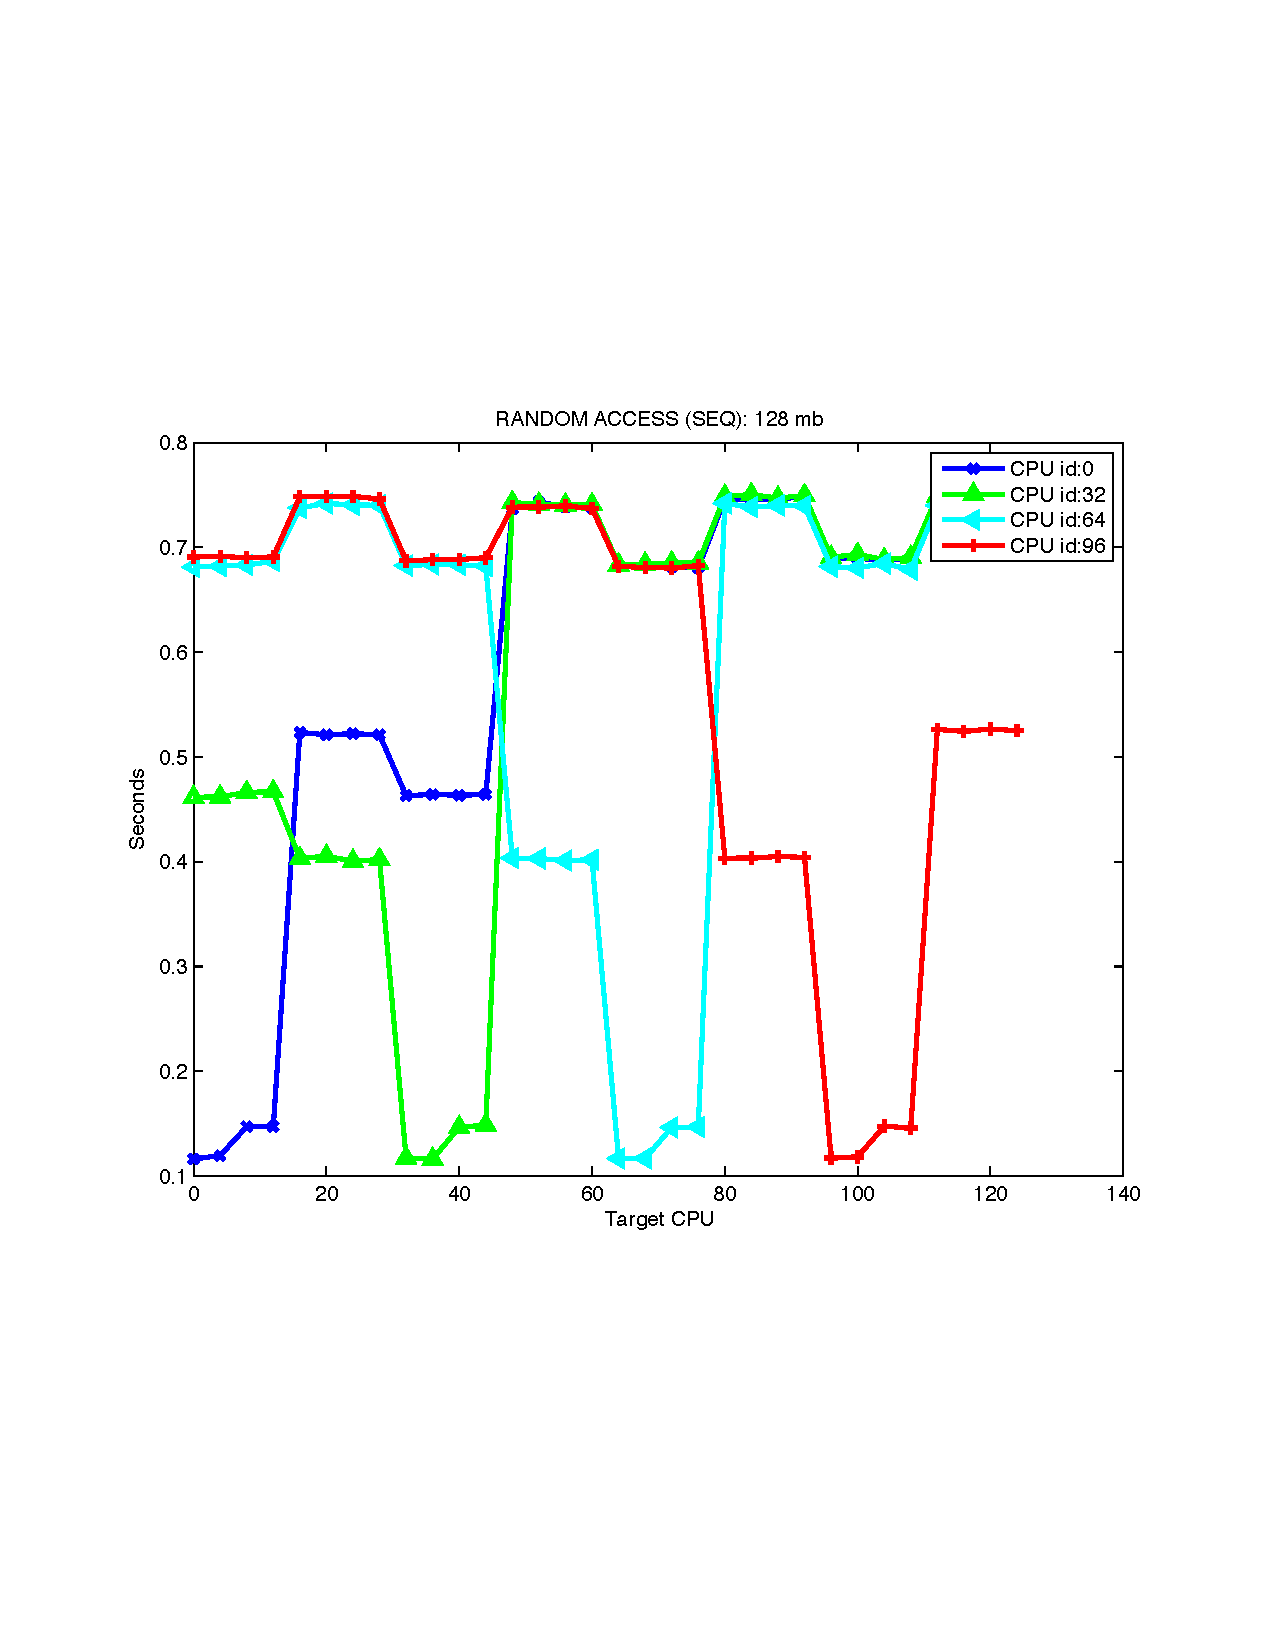
\includegraphics[width=0.95\textwidth]{blacklight_ranseq_access.pdf}
\caption{Sequential memory access experiment with random access pattern. Each cpu accesses the 128 megabyte array \emph{sparsely}, i.e jumping around it. 
}
\label{figseqran}
\end{figure}

\subsection{Experiment: Allocation}

Finally I measured the time for each allocation of 128 megabytes. All allocations were done in parallel. 
If memory was reallocated, I did not use realloc(), but first free() and then malloc(). The variation is quite
extreme, ranging from 1 seconds to 15 seconds. \textbf{This requires more study.}

\begin{figure}[H]
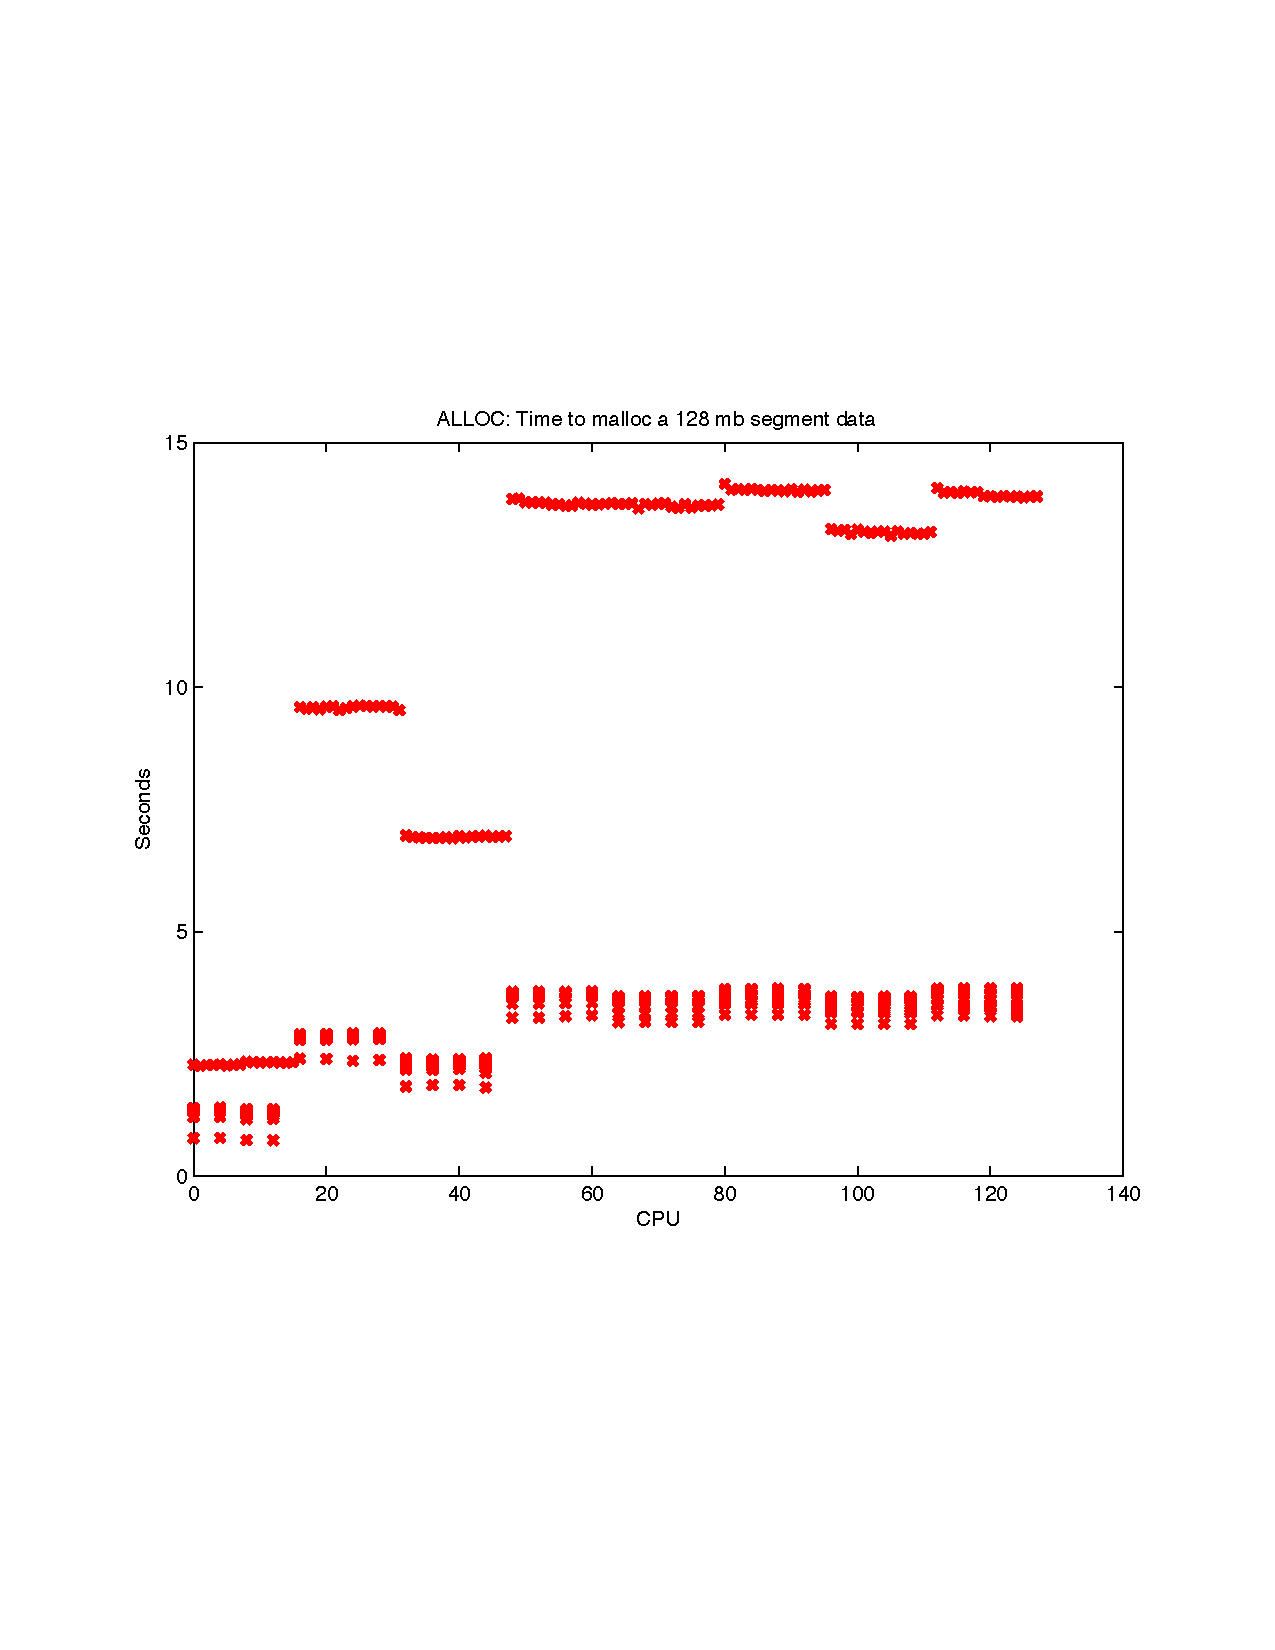
\includegraphics[width=0.95\textwidth]{blacklight_alloc_access.pdf}
\caption{Times for allocating 128 megabytes.
}
\label{figseqran}
\end{figure}


\subsection{Some conclusions}

These results show that remote reads can be over 5x slower than local reads. Moreover, they hint that
the memory system moves the data based on who uses it. This requires some more study, though.

Consider a CILK-type parallel "spawn" operation: 

\texttt{ spawn func (} \textit{data} \texttt{)}

An efficient spawn on Blacklight should take consideration the location of \textit{data} when
scheduling the execution. That is, it should prefer execution by a thread that is close to the data.


\section{Blacklight Experience So Far}

Job submission system in Blacklight is very easy to use and it is easy to transfer files back and forth using SVN or SCP.
Their support staff is very responsive by email (I had some account password issues).

I begun working on Blacklight Saturday, April 23. During this weekend, the task queue on Blacklight has been very long. 
The benchmark takes less than 10 minutes, but for a request of 128 cpus, I often need to wait for several hours. Sometimes,
like Monday morning April 27th, the jobs run almost instantly. Looking at the task queue, most jobs are scheduled to take 24-48 hours and when the queue is full, expected wait time is long. Yucheng Low told me that when he run jobs couple of weeks ago, they run almost instantly. Perhaps Blacklight is gaining traction and is thus overbusy.

 \end{document}
 
